\documentclass{beamer}


% Beamer settings
\usecolortheme{rose}
\beamertemplatenavigationsymbolsempty
\setbeamertemplate{footline}[frame number]

% Packages
\usepackage{amsmath}

\usepackage{pgfplots}
\usepgfplotslibrary{fillbetween}

\usepackage{minted}
\usepackage[T1]{fontenc} % Required by minted to ensure dollar signs are produced instead of pound (sterling) signs

\usepackage{multicol}

\usepackage{booktabs}


\title{A brief introduction to OpenMP}
\subtitle{1: Getting up to speed with OpenMP}

\begin{document}

\frame{\titlepage}

%-------------------------------------------------------------------------------
\section{OpenMP introduction}
\begin{frame}
\frametitle{What is OpenMP?}

A collection of compiler directives, library routines, and environment variables for parallelism for shared memory parallel programs.

\begin{itemize}
  \item Create and manage parallel programs while permitting portability.
  \item User-directed parallelization.
\end{itemize}

A \emph{specification} of annotations you can make to your program in order to make it parallel.

\end{frame}

%-------------------------------------------------------------------------------
\begin{frame}[fragile]
\frametitle{Syntax}
\begin{itemize}
\item OpenMP mostly formed of \emph{compiler directives}\\
  \begin{minted}{c}
  #pragma omp construct [clause [clause]...]
  \end{minted}
  These tell the compiler to insert some extra code on your behalf.

\item Compiler directives usually apply to a \emph{structured block} of statements.
Limited scoping in Fortran means we often need to use \emph{end} directives.
  \begin{minted}{c}
  #pragma omp construct
  {
    ... // lines of C code
  }
  \end{minted}

\item Library API calls
  \begin{minted}{c}
  #include <omp.h>
  omp_...();
  \end{minted}

\end{itemize}
\end{frame}

%-------------------------------------------------------------------------------
\subsection{Compiler flags}
\begin{frame}[fragile]
\frametitle{Building with OpenMP}

Turn on OpenMP in the compiler:
\begin{minted}{bash}
gcc *.c -fopenmp    # GNU
icc *.c -qopenmp    # Intel
\end{minted}

Can also build MPI and OpenMP programs by passing flags to \mintinline{c}|mpicc|.

\end{frame}

%-------------------------------------------------------------------------------
\section{Memory and execution model}
\begin{frame}
\frametitle{Shared memory}
OpenMP is for shared memory programming: all threads have access to a shared address space.

A typical HPC node consisting of 2 multi-core CPUs.
\begin{center}
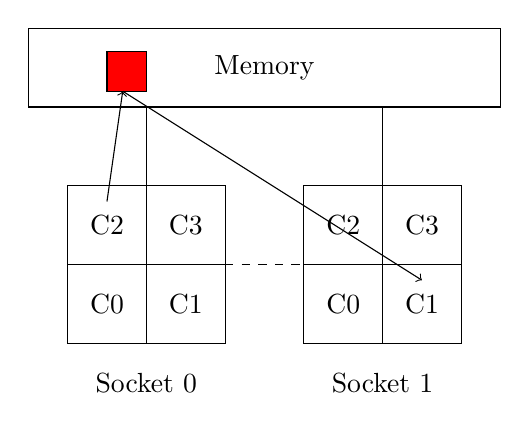
\begin{tikzpicture}
  % Draw 4 cores for socket 0
  \draw (0,0) rectangle (1,1);
  \draw (0.5,0.5) node {C0};
  \draw (1,0) rectangle (2,1);
  \draw (1.5,0.5) node {C1};
  \draw (0,1) rectangle (1,2);
  \draw (0.5,1.5) node {C2};
  \draw (1,1) rectangle (2,2);
  \draw (1.5,1.5) node {C3};
  \draw (1,-0.5) node {Socket 0};

  % Draw 4 cores for socket 1
  \draw (3,0) rectangle (4,1);
  \draw (3.5,0.5) node {C0};
  \draw (4,0) rectangle (5,1);
  \draw (4.5,0.5) node {C1};
  \draw (3,1) rectangle (4,2);
  \draw (3.5,1.5) node {C2};
  \draw (4,1) rectangle (5,2);
  \draw (4.5,1.5) node {C3};
  \draw (4,-0.5) node {Socket 1};

  % Draw large memory
  \draw (-0.5,3) rectangle (5.5,4);
  \draw (2.5,3.5) node {Memory};

  % Connect sockets to memory
  \draw (1,2) -- (1,3);
  \draw (4,2) -- (4,3);
  \draw[dashed] (2,1) -- (3,1); % QPI

  % Show memory shared
  \pause
  \draw[fill=red] (0.5,3.2) rectangle (1,3.7);
  \draw[->] (0.5,1.8) -- (0.7,3.2);
  \draw[->] (0.7,3.2) -- (4.5,0.8);

\end{tikzpicture}
\end{center}
\emph{All} threads (each running on a core) can access the same memory.

Different to MPI, where one process cannot see the memory of another without explicit communication.

\end{frame}

%-------------------------------------------------------------------------------
\begin{frame}
\frametitle{Fork-join model}
Serial/sequential execution:
\begin{center}
\begin{tikzpicture}
  \draw[->] (0,0) -- (8,0);
\end{tikzpicture}
\end{center}

\pause

In a \emph{fork-join} model, code starts serial, \emph{forks} a \emph{team} of threads then \emph{joins} them back to serial execution.
\begin{center}
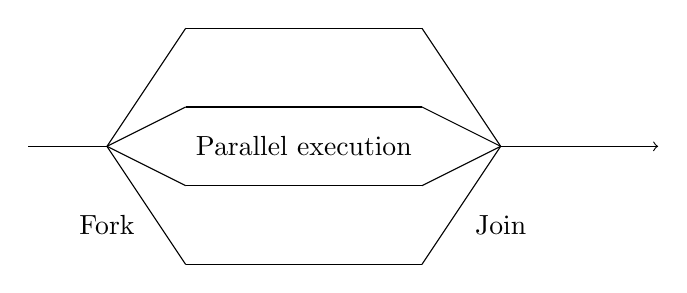
\begin{tikzpicture}
  \draw (0,0) -- (1,0);

  % Fork
  \draw (1,0) -- (2,1.5);
  \draw (1,0) -- (2,0.5);
  \draw (1,0) -- (2,-0.5);
  \draw (1,0) -- (2,-1.5);
  \draw (1,-1) node {Fork};

  % Run in parallel
  \draw (2,1.5)  -- (5,1.5);
  \draw (2,0.5)  -- (5,0.5);
  \draw (2,-0.5) -- (5,-0.5);
  \draw (2,-1.5) -- (5,-1.5);
  \draw (3.5,0) node {Parallel execution};

  % Join
  \draw (5,1.5)  -- (6,0);
  \draw (5,0.5)  -- (6,0);
  \draw (5,-0.5) -- (6,0);
  \draw (5,-1.5) -- (6,0);
  \draw (6,-1) node {Join};

  % Serial end
  \draw[->] (6,0) -- (8,0);
\end{tikzpicture}
\end{center}

Nested threads are allowed, where a thread forks its own team of threads.
\end{frame}

%-------------------------------------------------------------------------------
\section{Going parallel}
\begin{frame}[fragile]
\frametitle{Creating OpenMP threads}
\begin{minted}[frame=single, linenos]{c}

#pragma omp parallel
{
  printf("Hello\n");
}

\end{minted}

Threads \emph{redundantly} execute code in the block.

Each thread will output \mintinline{bash}|Hello|.

Threads are synchronised at the end of the parallel region.

\end{frame}

%-------------------------------------------------------------------------------
%\begin{frame}[fragile]
%\frametitle{Pthreads}
%
%\begin{minted}[fontsize=\small, linenos, frame=single]{fortran}
%program hello
%  use fpthread
%  integer :: i, err
%  integer :: N = 4
%  type(fpthread_t) :: Tide(N)
%
%  do i = 1, N
%    call fpthread_create(tid(i), NULL, run, NULL, err)
%  end do
%  do i = 1, N
%    call fpthread_join(tid(i), NULL, err)
%  end do
%
%  subroutine run
%    print *, "Hello"
%  end subroutine run
%end program hello
%\end{minted}
%
%\end{frame}
%
%%-------------------------------------------------------------------------------
%\begin{frame}
%\frametitle{OpenMP and Pthreads}
%\begin{itemize}
%  \item Pthreads is very error prone and verbose.
%  \item The OpenMP \mintinline{fortran}|!$omp parallel| abstracts this away.
%  \item The compiler directive inserts this extra code on your behalf.
%  \item Pthreads requires wrapping up your parallel work in subroutines.
%    \begin{itemize}
%      \item Kernels are a useful abstraction used in many programming models.
%    \end{itemize}
%  \item OpenMP much more convenient for \emph{incrementally} adding parallelism to your code.
%\end{itemize}
%\end{frame}

%-------------------------------------------------------------------------------
\begin{frame}[fragile]
\frametitle{Setting number of threads}
You might need to set the number of threads to launch (though typically you'll leave OpenMP to set the number of threads for you at run-time).

OpenMP has 3 ways to do this:
\begin{itemize}
  \item Environment variables
  \begin{minted}{bash}
  OMP_NUM_THREADS=16
  \end{minted}

  \item API calls
  \begin{minted}{c}
  omp_set_num_threads(16);
  \end{minted}

  \item Clauses
  \begin{minted}{c}
  #pragma omp parallel num_threads(16)
  {
  }
  \end{minted}
\end{itemize}

In general it's better to use environment variables if you need to do this, as this approach gives you more flexibility at runtime.
\end{frame}

%-------------------------------------------------------------------------------
\begin{frame}[fragile]
\frametitle{Thread API calls}
Most parallel programs are written in a SPMD style: \newline
{\bf S}ingle {\bf P}rogram, {\bf M}ultiple {\bf D}ata.
\begin{itemize}
  \item MPI has a SPMD model.
  \item Threads run the same code, and use their ID to work out which data to operate on.
\end{itemize}

The OpenMP API gives you calls to determine thread information when \emph{inside} a parallel region:
\begin{itemize}
  \item Get number of threads
    \begin{minted}{c}
    int nthreads = omp_get_num_threads();
    \end{minted}

  \item Get thread ID
    \begin{minted}{c}
    int tid = omp_get_thread_num();
    \end{minted}

\end{itemize}
\end{frame}

%-------------------------------------------------------------------------------
\section{Example: vector addition}
\begin{frame}[fragile]
\frametitle{Vector add}
Walkthrough parallelising vector addition using OpenMP.

\begin{minted}[fontsize=\footnotesize,linenos,frame=single]{c}
int main(void) {
  int N = 1024; // Length of array
  double *A, *B, *C; // Arrays

  // Allocate and initialise vectors
  A = malloc(sizeof(double)*N);
  B = malloc(sizeof(double)*N);
  C = malloc(sizeof(double)*N);
  for (int i = 0; i < N; ++i) {
    A[i] = 1.0; B[i] = 2.0; C[i] = 0.0;
  }

  // Vector add
  for (int i = 0; i < N; ++i)
    C[i] = A[i] + B[i];

  free(A); free(B); free(C);
}
\end{minted}
\end{frame}

%-------------------------------------------------------------------------------
\begin{frame}[fragile]
\frametitle{Vector add: Step 1}
Add parallel region around work
\begin{minted}[frame=single]{c}
  #pragma omp parallel
  {
    for (int i = 0; i < N; ++i)
      C[i] = A[i] + B[i];
  }
\end{minted}
Every thread will now do the entire vector addition --- redundantly!
\end{frame}

%-------------------------------------------------------------------------------
\begin{frame}[fragile]
\frametitle{Vector add: Step 2}
Get thread IDs
\begin{minted}[frame=single]{c}
  int tid, nthreads;

  #pragma omp parallel
  {
    tid = omp_get_thread_num();
    nthreads = omp_get_num_threads();

    for (int i = 0; i < N; ++i)
      C[i] = A[i] + B[i];
  }
\end{minted}

\pause
\begin{alertblock}{Incorrect behaviour at runtime}
What's the problem here?
\end{alertblock}
\end{frame}

%-------------------------------------------------------------------------------
\begin{frame}[fragile]
\frametitle{Vector add: Step 2, take 2}

\begin{itemize}
  \item In OpenMP, all variables are \emph{shared} between threads.
  \item But each thread needs its own copy of \mintinline{c}|tid|.
  \item Solution: use the \mintinline{c}|private| clause on the \mintinline{c}|parallel| region or declare variables inline.
  \item This gives each thread its own unique copy in memory for the variable.
\end{itemize}

\begin{minted}[frame=single]{fortran}


  #pragma omp parallel
  {
    int tid = omp_get_thread_num();
    int nthreads = omp_get_num_threads();

    for (int i = 0; i < N; ++i)
      C[i] = A[i] + B[i];
  }
\end{minted}
Much more information about data sharing clauses in next session.
\end{frame}

%-------------------------------------------------------------------------------
\begin{frame}[fragile]
\frametitle{Vector add: Step 3}
Finally, distribute the iteration space across the threads.
\begin{minted}[fontsize=\small,frame=single]{c}

  #pragma omp parallel
  {
    int tid = omp_get_thread_num();
    int nthreads = omp_get_num_threads();

    int i;
    for (i = tid*N/nthreads; i < (tid+1)*N/nthreads; ++i)
      C[i] = A[i] + B[i];
  }
\end{minted}
\begin{block}{Remember}
Thread IDs are numbered from 0 in OpenMP.
Be careful with your index calculation.
\end{block}
\end{frame}

%-------------------------------------------------------------------------------
\section{Worksharing}
\begin{frame}[fragile]
\frametitle{Worksharing}

\begin{itemize}
\item The SPMD approach requires lots of bookkeeping.
\item Common pattern of splitting loop iterations between threads.
\item OpenMP has worksharing constructs to help with this.
\item Used within a parallel region.
\item The loop iterator is made \mintinline{c}|private| by default: no need for data sharing clause.
\end{itemize}

\begin{minted}[frame=single]{c}
  int i;
  #pragma omp parallel
  {
    #pragma omp for
    for (i = 0; i < N; ++i) {
      C(i) = A(i) + B(i);
    } // End of for loop
  } // End of parallel region
\end{minted}

Implicit synchronisation point at the \mintinline{c}|} // End of for loop|.

\end{frame}

%-------------------------------------------------------------------------------
\begin{frame}[fragile]
\frametitle{Combined worksharing directives}
Generally it's convenient to combine the directives:
\begin{minted}[frame=single]{c}
#pragma omp parallel for
for (int i = 0; i < N; ++i) {
  ... // Loop body
}
\end{minted}

\begin{itemize}
  \item This starts a parallel region, forking some threads.
  \item Each thread then gets a portion of the iteration space and computes the loop body in parallel.
  \item Implicit synchronisation point at the \mintinline{c}|}|.
  \item Threads finally join again; later code executes sequentially.
\end{itemize}
\end{frame}

%-------------------------------------------------------------------------------
\begin{frame}
\frametitle{Taking stock}
\begin{itemize}
  \item We've seen how to parallelise a simple program using OpenMP.
  \item Shown the MPI-style SPMD approach for dividing work.
  \item OpenMP worksharing constructs make this easier.
\end{itemize}

The rest of this session:
\begin{itemize}
  \item Expands on the worksharing constructs.
  \item The first example for you to try.
\end{itemize}

Next time: the rest of the OpenMP common core.
\end{frame}

%-------------------------------------------------------------------------------
\section{Scheduling}
\begin{frame}[fragile]
\frametitle{The Schedule clause}
\begin{itemize}
  \item The worksharing clauses use default rules for assigning iterations to threads.
  \item Can use the \mintinline{c}|schedule| clause to specify the distribution.
  \item General format:
    \begin{minted}{c}
      #pragma omp parallel for schedule(...)
    \end{minted}
\end{itemize}
Next slides go through the options, using the following loop as an example:
\begin{minted}[frame=single]{c}
#pragma omp parallel do num_threads(4)
for (int i = 0; i < 100; ++i) {
  ... // loop body
}
\end{minted}

\end{frame}

%-------------------------------------------------------------------------------
\begin{frame}[fragile]
\frametitle{Static schedule}
\begin{minted}{c}
schedule(static)
schedule(static,16)
\end{minted}

\begin{itemize}
\item Static schedule divides iterations into chunks and assigns chunks to threads in round-robin.
\item If no chunk size specified, iteration space divided roughly equally.
\end{itemize}
For our example loop:
\begin{columns}
\begin{column}{0.5\textwidth}
  \mintinline{c}|schedule(static)|
  \begin{tabular}{cc}
  \toprule
  Thread ID & Iterations \\
  \midrule
  0 &  1--25 \\
  1 & 26--50 \\
  2 & 51--75 \\
  3 & 76--100 \\
  \bottomrule
  \end{tabular}
\end{column}

\begin{column}{0.5\textwidth}
  \mintinline{c}|schedule(static,16)|
  \begin{tabular}{cc}
  \toprule
  Thread ID & Iterations \\
  \midrule
  0 &  1--16, 65--80 \\
  1 & 17--32, 81--96 \\
  2 & 33--48, 97--100 \\
  3 & 49--64 \\
  \bottomrule
  \end{tabular}
\end{column}
\end{columns}

\end{frame}

%-------------------------------------------------------------------------------
\begin{frame}[fragile]
\frametitle{Dynamic schedule}
\begin{minted}{c}
schedule(dynamic)
schedule(dynamic,16)
\end{minted}

\begin{itemize}
  \item Iteration space is divided into chunks according to chunk size.
  \item If no chunk size specified, default size is one.
  \item Each thread requests and executes a chunk, until no more chunks remain.
  \item Useful for unbalanced work-loads if some threads complete work faster.
\end{itemize}

For our example with a chunk size of 16:
\begin{itemize}
  \item The iteration space is split into chunk of 16 (the last chunk may be smaller).
  \item Each threads gets one chunk, then requests a new chunk to work on.
\end{itemize}

\end{frame}

%-------------------------------------------------------------------------------
\begin{frame}[fragile]
\frametitle{Guided schedule}
\begin{minted}{c}
schedule(guided)
schedule(guided,16)
\end{minted}

\begin{itemize}
  \item Similar to assignment to dynamic, except the chunk size decreases over time.
  \item Granularity of work chunks gets finer over time.
  \item If no chunk size is specified, the default size is one.
  \item Useful to try to mitigate overheads of a \mintinline{c}|dynamic| schedule by starting with large chunks of work.
\end{itemize}

For our example with a chunk size of 16:
\begin{itemize}
  \item Each thread gets a chunk of 16 to work on.
  \item Each thread requests a new chunk, which might be smaller than 16.
\end{itemize}

\end{frame}

%-------------------------------------------------------------------------------
\begin{frame}[fragile]
\frametitle{Other schedules}
\begin{minted}{c}
schedule(auto)
\end{minted}
\begin{itemize}
  \item Let the compiler or runtime choose the schedule.
\end{itemize}

\vfill

\begin{minted}{c}
schedule(runtime)
\end{minted}
\begin{itemize}
  \item Get the schedule from the \mintinline{bash}|OMP_SCHEDULE| environment variable.
\end{itemize}

\begin{block}{Recommendation}
Just use a \mintinline{c}|static| schedule unless there is a good reason not to!
\mintinline{c}|static| is usually the fastest of all the options.
The choice of schedules is an advanced tuning option.
\end{block}

\end{frame}

%-------------------------------------------------------------------------------
\section{Loops}
\begin{frame}[fragile]
\frametitle{Nested loops}
\begin{itemize}
  \item Often have tightly nested loops in your code.
  \item E.g. 2D grid code, every cell is independent.
  \item OpenMP worksharing would only parallelise over first loop with each thread performing inner loop serially.
  \item Use the \mintinline{c}|collapse(...)| clause to combine iteration spaces.
  \item OpenMP then workshares the combined iteration space.
\end{itemize}

\begin{minted}[frame=single]{c}
#pragma omp parallel for collapse(2)
for (int i = 0; i < N; ++i) {
  for (int j = 0; j < N; ++j) {
    ... // loop body
  }
}
\end{minted}
All $N^2$ iterations are distributed across threads, rather than just the $N$ of the outer loop.

\end{frame}


%-------------------------------------------------------------------------------
\begin{frame}
\frametitle{Nested loops}
\begin{block}{Performance note}
Collapsing loops may subtly effect the compiler's knowledge about alignment and could affect vectorisation.
More on this when we talk about vectorisation in a later session.
\end{block}

\end{frame}

%-------------------------------------------------------------------------------
\section{Synchronisation}
\begin{frame}[fragile]
\frametitle{The nowait clause}
\begin{itemize}
  \item May have series of loops in your code which are independent.
  \item Threads must wait/synchronise at the end of the loop.
  \item But it might be possible to delay this synchronisation using the \mintinline{c}|nowait| clause.
  \item When a thread finishes the first loop, it starts on the next loop.
\end{itemize}

\begin{minted}[fontsize=\small, linenos, frame=single]{c}
#pragma omp parallel
{
#pragma omp for nowait
for (int i = 0; i < N; ++i) {
  A[i] = i;
} // No barrier!

#pragma omp for
for (int i = 0; i < N; ++i) {
  B[i] = i;
} // Implicit barrier
} // Implicit barrier
\end{minted}
\end{frame}

%-------------------------------------------------------------------------------
% \begin{frame}
% \frametitle{Synchronisation}
% A number of ways to synchronise the threads in OpenMP:
% \begin{multicols}{2}
% \begin{itemize}
%   \item Barriers
%   \item Critical
%   \item Atomics
%   \item Locks
%   \item Ordered
%   \item Single
%   \item Master
%   \item Flush
% \end{itemize}
% \end{multicols}
% 
% \vfill
% 
% \begin{itemize}
%   \item Will look at Critical and Atomic in Session 2.
%   \item Ordered, Single and Master in Session 6.
%   \item Won't formally cover Flush and Locks --- advanced stuff with esoteric use cases.
% \end{itemize}
% 
% Quickly cover barriers now.
% 
% \end{frame}
%
%-------------------------------------------------------------------------------
\begin{frame}[fragile]
\frametitle{Barriers}
A barrier simply synchronises threads in a parallel region.

\begin{minted}[frame=single,linenos]{c}
#pragma omp parallel
{

int tid = omp_get_thread_num();
A[tid] = big_work1(tid);

#pragma omp barrier

B[tid] = big_work2(A, tid);

}
\end{minted}

\begin{itemize}
  \item Running in parallel, need to compute \mintinline{c}|A[]| before computing \mintinline{c}|B[]|.
  \item The barrier ensures all threads wait between these statements.
  \item Must ensure all threads encounter the barrier.
\end{itemize}

\end{frame}

%-------------------------------------------------------------------------------
\section{Miscellaneous}
%\begin{frame}[fragile]
%\frametitle{Nested threads}
%\begin{itemize}
%  \item Turn on support with by setting the environment variable \mintinline{c}|OMP_NESTED=true|, otherwise inner region is default serial.
%  \item Every thread in the (outer) parallel region then spawns threads.
%  \item Control the number of threads with clauses or environment variable: \mintinline{bash}|OMP_NUM_THREADS=4,2|.
%\end{itemize}
%
%\begin{minted}[frame=single]{c}
%#pragma omp parallel num_threads(4)
%{
%  ... // A parallel region
%  #pragma omp parallel num_threads(4)
%  {
%    ... // Inner parallel region
%  }
%}
%\end{minted}
%
%\end{frame}
%
%
%-------------------------------------------------------------------------------
%\begin{frame}
%\frametitle{Nested threads}
%\begin{alertblock}{Warning!}
%Be careful how you use nesting threads.
%It's very easy to oversubscribe threads.
%Thread affinity can be tricky.
%You probably don't need to use nested threads!
%\end{alertblock}
%\end{frame}
%
%-------------------------------------------------------------------------------
\begin{frame}[fragile]
\frametitle{Multi-line directives}
\begin{itemize}
  \item Sometimes OpenMP directives can be quite long.
  \item Nicer to split up the directive across lines in the source file using line continuation character \mintinline{c}|\|:
\end{itemize}

\begin{minted}{c}
#pragma omp construct \
clause \
clause
\end{minted}

\end{frame}

%-------------------------------------------------------------------------------
\begin{frame}
\frametitle{Summary}
This section introduced the OpenMP programming model:
\begin{itemize}
  \item Creating parallel regions: \mintinline{c}{pragma omp parallel}
  \item Getting thread IDs: \mintinline{c}{omp_get_thread_num()}/\mintinline{c}{omp_get_num_threads()}
  \item Worksharing constructs: \mintinline{c}{pragma omp for}
  \item The \mintinline{c}|schedule| and \mintinline{c}{nowait} clauses
  \item Synchronising threads with barriers: \mintinline{c}{pragma omp barrier}
\end{itemize}
\end{frame}

%-------------------------------------------------------------------------------
 \begin{frame}
 \frametitle{Resources}
 \begin{itemize}
 \item OpenMP website: \url{https://www.openmp.org}
   \begin{itemize}
     \item The specification (not for the faint hearted).
     \item Download summary cards.
     \item List of compiler support.
     \item Example code for all the directives.
     \item List of books: \url{https://www.openmp.org/resources/openmp-books/}
   \end{itemize}
 
 \item cOMPunity
   \begin{itemize}
     \item \url{http://www.compunity.org}
   \end{itemize}
 
 \item Online tutorials:
   \begin{itemize}
     \item Tim Mattson's YouTube tutorial: \url{https://youtu.be/nE-xN4Bf8XI}
     \item SC'08 tutorial from Tim Mattson and Larry Meadows: \url{https://openmp.org/mp-documents/omp-hands-on-SC08.pdf}
     \item From Lawrence Livermore National Lab: \url{https://computing.llnl.gov/tutorials/openMP/}
   \end{itemize}
 
 \end{itemize}
 
 \end{frame}

%-------------------------------------------------------------------------------

\end{document}
